\documentclass[11pt,a4paper]{article}
\usepackage[utf8]{inputenc}
\usepackage[T1]{fontenc}
\usepackage{lmodern}
\usepackage[margin=2.5cm]{geometry}
\usepackage{graphicx}
\usepackage{booktabs}
\usepackage{amsmath}
\usepackage{microtype}
\usepackage[hidelinks]{hyperref}
\usepackage{listings}
\usepackage{caption}
\captionsetup{font=small,labelfont=bf}
\lstset{
  basicstyle=\ttfamily\footnotesize,
  breaklines=true,
  frame=single,
  framesep=4pt,
  xleftmargin=6pt,
  xrightmargin=6pt,
  columns=fullflexible,
  keepspaces=true
}
\title{\textbf{Tabular Datasets for the Posttraining Pipeline of Apertus}\\[1ex]
\large Semester Project Report -- Spring 2026}
\author{Dijana Janjetovic\\[0.5ex]
\small Supervisor: Prof.\ Antoine Bosselut}
\date{June 2026}
\begin{document}
\maketitle
\begin{abstract}
\noindent
Apertus, the open-weight Swiss large language model (LLM)~\cite{apertus}, is adding tabular data to its posttraining mixture. Because a language model reads a flat token sequence rather than a two-dimensional grid, every table must first be serialized into text, and that choice determines which structure the model can learn. Prior work on serialization addresses fine-tuning and in-context learning rather than posttraining at scale~\cite{tabllm,jaitly,wang,wu2025}. We present a controlled ablation over five serialization formats (key:value, CSV, Markdown, JSON, and a novel SQL-schema-annotated format) in which data, architecture, and data order are held consistent. For each format, 1.54B-parameter proxy models are trained on serialized tables from the T4 corpus~\cite{t4} on CSCS Alps for two random seeds, and evaluated with a BLiMP-style minimal-pair protocol~\cite{blimp} comprising 1{,}496 statement pairs. Comparing formats at matched rows seen and averaging over seeds, the leading formats (CSV, JSON, SQL schema, and Markdown) are statistically indistinguishable on overall accuracy, all within noise of the 50\% chance baseline, while key:value performs worst; an initial single-seed exploration had suggested a CSV/JSON advantage that does not persist under replication. Together with CSV's approximately twofold token-efficiency advantage over record-style formats, and its accuracy-neutrality within the leading group, the evidence supports CSV as the serialization format for Apertus tabular posttraining. Hence, the complete T4 corpus has been serialized and tokenized accordingly. We conclude with the further analyses required to consolidate these findings.
\end{abstract}
\section{Introduction}
Apertus is an open-weight LLM developed by the Swiss AI Initiative and trained on the Alps supercomputer at CSCS~\cite{apertus}. Its forthcoming iteration extends posttraining with additional modalities, including structured tabular data. Tables underlie a substantial fraction of real-world information (databases, spreadsheets, financial and scientific records), and reliable reasoning over them enables a correspondingly broad class of downstream tasks.
Incorporating tables into a text-based posttraining pipeline raises a deceptively simple question: in what textual form should a table be presented to the model? A transformer observes a one-dimensional token sequence rather than a two-dimensional grid, and the serialization format therefore determines which structural cues (column boundaries, header semantics, row delimitation) are available to be learned. The choice is consequential, as downstream performance on tabular benchmarks varies by several percentage points depending on the alignment between inference-time input formats and formats encountered during training~\cite{wu2025}.
Existing studies of table serialization concern few-shot classification, fine-tuning, or in-context learning~\cite{tabllm,jaitly,wang,ono}, and corpora derived from TabLib~\cite{tablib}, such as T4~\cite{t4}, serialize tables as classification-task wrappers unsuited to general next-token posttraining. To our knowledge, no controlled comparison of serialization formats for \emph{posttraining} has been published. This project addresses that gap. Our contributions are: (i)~a reproducible pipeline on CSCS Alps that converts raw T4 Parquet tables into Megatron-ready training data in five formats, including a segmentation scheme (\emph{tabular chunking}) that retains every row of every table; (ii)~a novel SQL-schema-annotated serialization for posttraining, derived at negligible cost from Parquet metadata; (iii)~a controlled five-way ablation with 1.54B-parameter proxy models trained under identical conditions and replicated across two seeds; (iv)~a minimal-pair evaluation with per-pair and per-table scoring and a table-difficulty consistency analysis; and (v)~a format recommendation together with a fully serialized and tokenized T4 corpus ready for the Apertus data mixture.
\section{Related Work}
TabLib~\cite{tablib} comprises 627M tables extracted from GitHub and Common Crawl; T4~\cite{t4} filters it to approximately 3.1M high-quality tables (roughly 100B tokens), handling deduplication, PII removal, and language filtering, but leaving tables as raw two-dimensional cell values. Serialization templates for LLMs were introduced primarily for few-shot classification; TabLLM~\cite{tabllm} established the key:value sentence template, and subsequent studies compare templates in fine-tuning and in-context settings~\cite{jaitly,wang,ono}. \texttt{CREATE TABLE} schema prompts are standard in the text-to-SQL literature~\cite{spider,wu2025}, where the survey of Wu et al.~\cite{wu2025} notes that the effectiveness of alternative table representations beyond retrieval-style tasks remains under-investigated; their use as a posttraining serialization is unexplored. Our evaluation adapts BLiMP~\cite{blimp}, which scores minimal pairs by model likelihood without fine-tuning, and our proxy-model methodology follows the scaling-law practice of selecting design choices at small scale~\cite{chinchilla}.
\section{Method}
\label{sec:design}
\subsection{Serialization formats}
Five formats were selected to span the spectrum from compact to verbose and from implicit to explicit structure. Illustrated on a small example table:
\paragraph{A -- key:value (baseline~\cite{tabllm,t4}).}\mbox{}
\begin{lstlisting}
The city is Zurich. The population is 0.42. The area is 88.
The city is Geneva. The population is 0.20. The area is 16.
\end{lstlisting}
\paragraph{B -- CSV.}\mbox{}
\begin{lstlisting}
city, population, area
Zurich, 0.42, 88
Geneva, 0.20, 16
\end{lstlisting}
\paragraph{C -- Markdown.} Pipe-delimited rows with a separator line, the form most frequently encountered during text training (GitHub, Wikipedia); alignment padding and the separator row incur token overhead.\mbox{}
\begin{lstlisting}
| city   | population | area |
|--------|------------|------|
| Zurich | 0.42       | 88   |
| Geneva | 0.20       | 16   |
\end{lstlisting}
\paragraph{D -- JSON.}\mbox{}
\begin{lstlisting}
[{"city": "Zurich", "population": 0.42, "area": 88},
 {"city": "Geneva", "population": 0.20, "area": 16}]
\end{lstlisting}
\paragraph{E -- SQL schema (novel format).}\mbox{}
\begin{lstlisting}
CREATE TABLE data (
    city VARCHAR,
    population FLOAT,  -- range: 0.13 to 0.42
    area INT           -- range: 16 to 88
);
city, population, area
Zurich, 0.42, 88
Geneva, 0.20, 16
\end{lstlisting}
A \texttt{CREATE TABLE} header with column types and value ranges, inferred directly from Parquet column statistics, precedes compact CSV rows. The format exploits the model's prior exposure to SQL~\cite{spider} and is hypothesized to be most beneficial for tables whose column names carry little semantic content (e.g.\ \texttt{col\_1}, \texttt{value}), which survive T4's filtering in non-trivial numbers.
\subsection{Serialization design}
In contrast to T4's one-row-per-sample classification setup~\cite{t4}, each training sample packs as many rows of a single table as fit a 3{,}800-token budget (the remainder of the 4{,}096-token context being reserved for special tokens), enabling the model to learn cross-row regularities. Tables exceeding the budget are split into multiple segments by greedy row accumulation with per-row token pre-computation (\emph{tabular chunking}); every segment repeats the header or schema, and no row is discarded. Rows are shuffled deterministically with a filename-derived seed so that all five format variants observe identical row orderings, removing data order as a confound. Cleaning removes artifact columns (\texttt{Unnamed:*}, \texttt{index}), all-null columns, and columns containing cells longer than 500 characters.
\subsection{Pipeline and training setup}
The pipeline executes on CSCS Alps (Clariden) in four phases\footnote{Code: \url{https://github.com/janjetovicd/local-tabular-pretraining} and \url{https://github.com/janjetovicd/tabular_ablation}. Training used the SwissAI Megatron-LM fork, branch \texttt{feat/new-phase}, commit \texttt{b870127a2}.}: (1)~serialization of T4 chunks 0--23 via SLURM array jobs, producing a multi-format corpus far larger than the 30B-token training budget, so each run makes less than a single pass over its data; (2)~tokenization with the Apertus BPE tokenizer (128k vocabulary) into Megatron binary format using datatrove's \texttt{MegatronDocumentTokenizer}; (3)~training of five proxy models, replicated across two seeds, with the SwissAI fork of Megatron-LM~\cite{megatron}; and (4)~evaluation on held-out chunks 24--25. Two operational findings merit documentation: Clariden compute nodes lack internet access, so the tokenizer must be pre-cached on the login node, and Megatron's \texttt{preprocess\_data.py} silently produces empty output under this restriction, whereas datatrove with a cached tokenizer path does not.
Training Apertus itself five times would be computationally prohibitive; following standard scaling-law methodology~\cite{chinchilla}, the ablation study therefore employs proxy models of the same architectural family, under the assumption that the relative ranking of formats transfers across scale. Table~\ref{tab:model} summarizes the configuration; all runs share schedule and data order, leaving serialization format as the sole independent variable. Because denser formats pack roughly twice as many rows per token (Table~\ref{tab:tokens}), comparing formats at a fixed token budget would grant CSV and SQL schema about twice the table content. Formats are therefore compared not at a fixed number of tokens but at the checkpoint where each has processed the same number of table rows, which removes this data-exposure advantage. Each run trains a fixed budget of 30B tokens, approximately 20 tokens per parameter and thus close to the compute-optimal ratio for a 1.54B model~\cite{chinchilla}.
\begin{table}[ht]
\centering
\small
\begin{tabular}{llll}
\toprule
\multicolumn{2}{c}{\textbf{Architecture}} & \multicolumn{2}{c}{\textbf{Training}}\\
\cmidrule(lr){1-2}\cmidrule(lr){3-4}
Layers & 32 & Tokens per run & $\sim$30B\\
Hidden / FFN size & 2{,}048 / 6{,}144 & Global batch & 256 $\times$ 4{,}096 tokens\\
Heads & 16 (GQA~\cite{gqa}, 4 KV) & Optimizer & Adam ($\beta_1{=}0.9$, $\beta_2{=}0.95$)\\
Parameters & 1.54B + 524M emb. & Learning rate & $3\mathrm{e}{-4}$ cosine $\rightarrow 3\mathrm{e}{-5}$\\
Positional encoding & RoPE~\cite{rope} & Precision & bfloat16\\
Normalization & RMSNorm & Seeds / hardware & 2 seeds; 32$\times$ GH200, $\sim$12\,h\\
\bottomrule
\end{tabular}
\caption{Proxy-model architecture and training configuration.}
\label{tab:model}
\end{table}
\subsection{Evaluation protocol}
\label{sec:eval}
From held-out chunks, 299 tables were sampled (each with at least two rows and a header fitting the token budget in all five formats). To remove the truncation artifact at its source, each table is first truncated to the 3{,}800-token context budget; LLaMA-3.1-8B-Instruct~\cite{llama3} is then prompted \emph{on that already-truncated context} to generate one factually correct statement and one plausible distractor for each of five task types (lookup, aggregation, comparison, inference, and multihop), yielding 1{,}496 minimal pairs per format (roughly five per table). Because each statement is generated from exactly the context the proxy model later scores against, the cell required to verify it can never be truncated away at scoring time. Identical statement pairs are used across formats, so generation noise cannot bias the ranking. Each proxy model scores both statements by mean negative log-likelihood (NLL) conditioned on the table context; a pair is correct when the true statement receives the higher likelihood. The protocol is a binary forced choice (chance: 50\%) requiring neither labels nor fine-tuning, in the manner of BLiMP~\cite{blimp}. Following feedback from the project review, accuracy is reported in two complementary ways rather than broken down by task type. \emph{Per-pair accuracy} is the percentage of individual statement/distractor pairs scored correctly. \emph{Per-table accuracy} aggregates the (up to five) pairs belonging to each table: the all-correct variant is the percentage of tables for which every pair is correct, and the majority variant is the percentage of tables for which more than half of the pairs are correct (at least three of five). All three quantities are expressed in percent.
\section{Results}
\paragraph{Token efficiency.} Measured over 200 sampled tables (Table~\ref{tab:tokens}), CSV and SQL schema accommodate approximately twice as many rows per sample as key:value and JSON; the schema header costs only ${\sim}3\%$ of rows relative to plain CSV. For a fixed training token budget, higher row density translates directly into more unique tabular content observed by the model, which is precisely why the formats are compared at matched rows seen rather than at matched tokens.
\begin{table}[ht]
\centering
\small
\begin{tabular}{lcc}
\toprule
\textbf{Format} & \textbf{Avg.\ rows/sample} & \textbf{Relative to key:value}\\
\midrule
key:value (baseline) & 30.7 & 1.00$\times$\\
JSON & 29.9 & 0.97$\times$\\
Markdown & 50.9 & 1.66$\times$\\
SQL schema & 58.2 & 1.90$\times$\\
CSV & 59.9 & 1.95$\times$\\
\bottomrule
\end{tabular}
\caption{Token efficiency over 200 tables (context 4{,}096; budget 3{,}800).}
\label{tab:tokens}
\end{table}
\paragraph{Training dynamics.} All runs converge stably over ${\sim}29$k steps (Figure~\ref{fig:loss}). The verbose formats (JSON, key:value, Markdown) attain \emph{lower} final training loss than CSV and SQL schema. This reflects the greater predictability of repetitive token streams rather than superior table understanding; training loss is therefore not a valid selection criterion, motivating the downstream evaluation. Brief upward spikes in some curves are checkpoint-reload artifacts and recover within a few hundred steps.
\begin{figure}[ht]
\centering
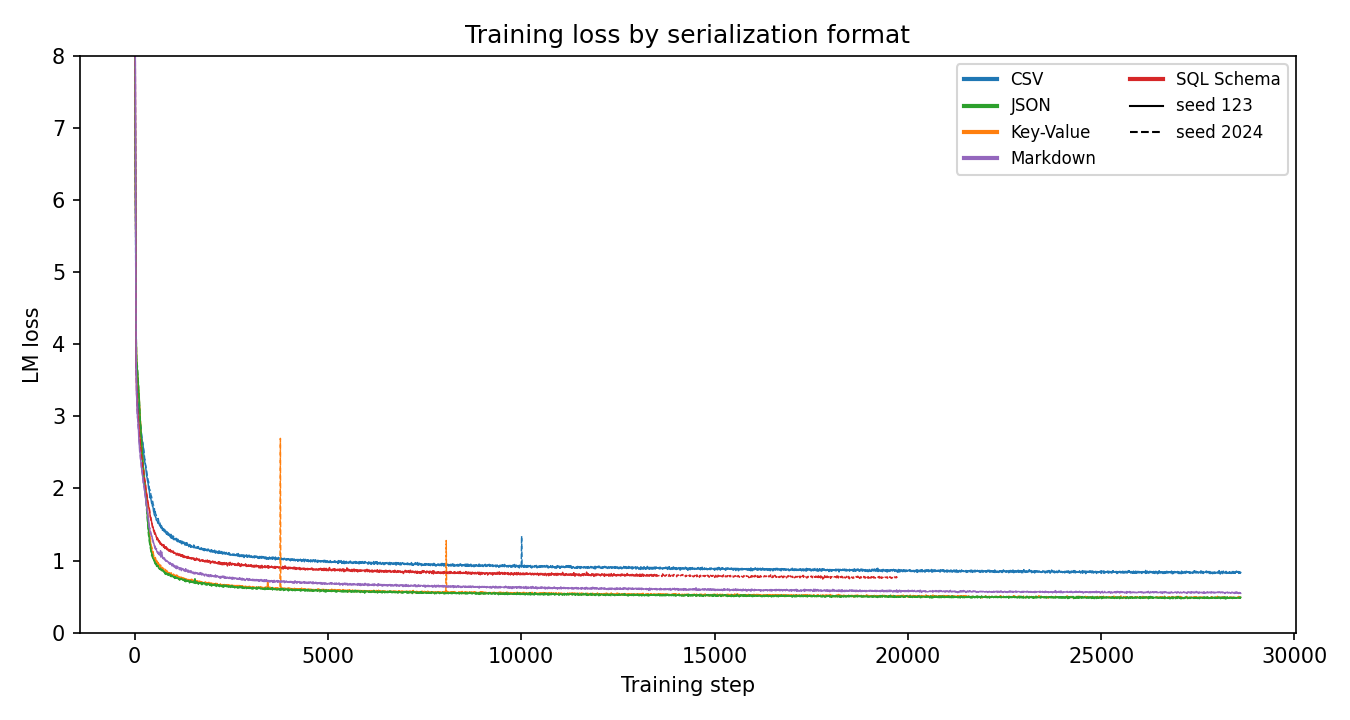
\includegraphics[width=0.95\textwidth]{loss_curves_v2.png}
\caption{Training loss by serialization format, for both random seeds (solid: seed 123; dashed: seed 2024). Verbose formats (JSON, key:value, Markdown) reach lower loss because their token streams are more predictable, not because the resulting models are better, which is why training loss is not used to select a format. Brief upward spikes are checkpoint-reload artifacts. Runs were checkpoint-restarted after preemption, so the SQL schema curves end near step 20{,}000; all formats had plateaued well before this.}
\label{fig:loss}
\end{figure}
\paragraph{Minimal-pair accuracy.} Table~\ref{tab:results} reports accuracy on the common evaluation set (1{,}484 pairs that every format could serialize), averaged over the two seeds. No format separates on overall accuracy: CSV, JSON, SQL schema, and Markdown lie within noise of one another and of chance, while key:value is significantly the weakest. To make ``within noise'' precise, each format's accuracy is treated as a binomial proportion and compared using the normal approximation. The standard error of a single format's accuracy is
\begin{equation}
\mathrm{SE}_p \;=\; \sqrt{\frac{p\,(1-p)}{n}} \;=\; \sqrt{\frac{0.5\,(1-0.5)}{1484}} \;\approx\; 1.30\%,
\label{eq:se}
\end{equation}
where $p$ is the chance accuracy ($p=0.5$, the value that maximises the variance $p(1-p)$, giving a conservative bound) and $n$ is the number of scored pairs per format ($n=1484$). Comparing two formats uses the standard error of the \emph{difference} of two approximately independent proportions,
\begin{equation}
\mathrm{SE}_{\Delta} \;=\; \sqrt{\mathrm{SE}_{p,1}^{2}+\mathrm{SE}_{p,2}^{2}} \;=\; \sqrt{2}\,\mathrm{SE}_p \;\approx\; 1.84\%,
\label{eq:sediff}
\end{equation}
and a difference $\Delta$ between two formats is significant at the $95\%$ level only if
\begin{equation}
|\Delta| \;>\; z_{0.975}\,\mathrm{SE}_{\Delta} \;=\; 1.96 \times 1.84\% \;\approx\; 3.6\ \text{percentage points},
\label{eq:thresh}
\end{equation}
where $z_{0.975}=1.96$ is the two-sided critical value of the standard normal distribution at the $95\%$ confidence level. By this criterion the four leading formats, which span only about 2.7 percentage points and whose per-seed ranking is unstable, are indistinguishable; key:value trails the leaders by 3.5 to 5.1 percentage points and is significantly worse. Because the same statement pairs are scored across all formats, a paired test (e.g.\ McNemar's) would be marginally more sensitive; the independent-samples bound of Eq.~\eqref{eq:thresh} is therefore conservative. The per-table ``all correct'' rates near 4\% match the chance expectation of all five pairs landing correct ($0.5^5=3.1\%$), an internal check confirming the models sit at chance per pair on most tables. An initial single-seed exploration (seed~42) had suggested a CSV/JSON advantage, but it does not persist once seed variance and equal rows seen are accounted for.
\begin{table}[ht]
\centering
\small
\begin{tabular}{lccc}
\toprule
\textbf{Format} & \textbf{Per-pair} & \textbf{Per-table (all)} & \textbf{Per-table (majority)}\\
\midrule
SQL schema & \textbf{53.0} & 4.2 & \textbf{57.7}\\
CSV & 51.4 & \textbf{4.4} & 53.7\\
JSON & 51.4 & 4.2 & 54.2\\
Markdown & 50.3 & 3.2 & 51.3\\
key:value & 47.9 & 3.7 & 46.5\\
\bottomrule
\end{tabular}
\caption{Minimal-pair accuracy (\%) on the common 1{,}484-pair set (the 12 of 1{,}496 pairs whose SQL schema table failed to serialize are excluded from every format so the denominators match), mean of the two seeds (chance $=50\%$). Per-pair, per-table all-correct, and per-table majority accuracy are defined in Section~\ref{sec:eval}.}
\label{tab:results}
\end{table}
\paragraph{Answerability (truncation control).} A truncation artifact would arise if the cell required to verify a statement were pushed out of the context window, so that no format could answer regardless of serialization. This is eliminated by construction: each table is truncated to the context budget \emph{before} statement generation (Section~\ref{sec:eval}), so every statement is answerable from the exact context the model scores against. The artifact is therefore removed at its source rather than corrected after the fact, and it no longer depresses the lookup and aggregation cases as it did in earlier, non-truncated evaluation runs.
\paragraph{Consistency across formats.} To test whether the near-chance result reflects a weak model or intrinsically hard tables, per-table accuracy was correlated across seeds and across formats (Figure~\ref{fig:consistency}). Here correlation is the Pearson correlation coefficient $r$, a dimensionless quantity ranging from $-1$ (perfect disagreement) to $+1$ (perfect agreement), with $0$ indicating no linear relationship. Cross-format coefficients of $r=0.41$--$0.61$ show that the formats fail on the \emph{same} tables, so per-table difficulty is a property of the table and its distractors rather than of the serialization format; cross-seed coefficients of $r=0.29$--$0.50$ confirm the difficulty is repeatable, and a stable easy tail of tables reaches 78--86\% accuracy across all formats, showing the models did learn. The evaluation therefore measures table and distractor difficulty more than serialization quality, which is why the leading formats cannot be separated on accuracy.
\begin{figure}[ht]
\centering
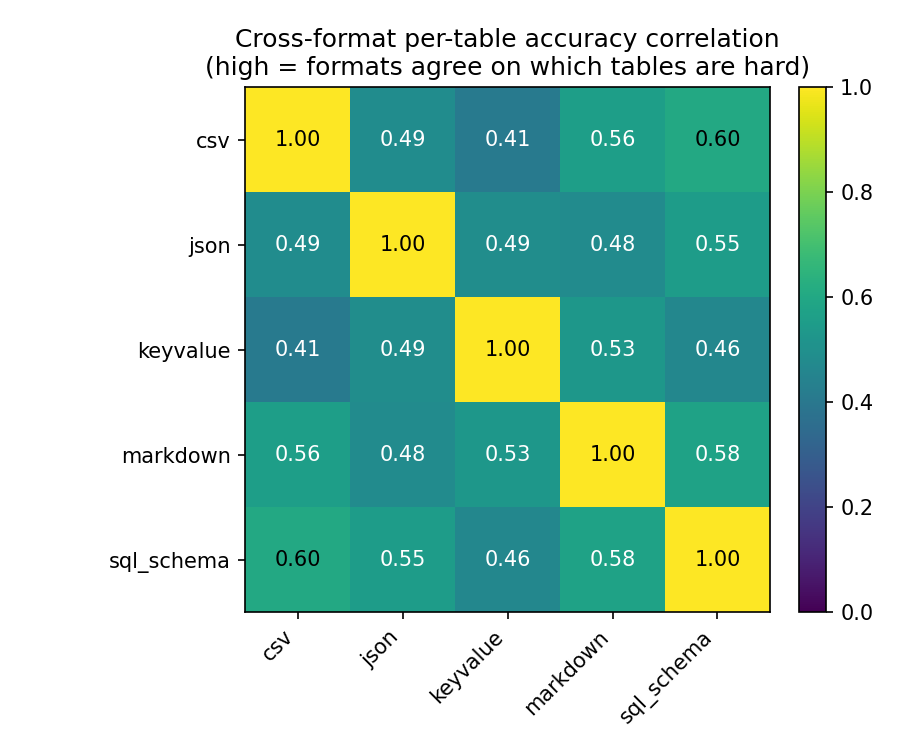
\includegraphics[width=0.6\textwidth]{consistency_heatmap.png}
\caption{Cross-format correlation of per-table accuracy. High off-diagonal values indicate that all formats fail on the same tables, pointing to the evaluation rather than the format.}
\label{fig:consistency}
\end{figure}
\section{Discussion}
\label{sec:discussion}
\paragraph{Recommendation.} Two converging observations support serializing Apertus tabular data as CSV. First, CSV is approximately twice as token-efficient as JSON and key:value (Table~\ref{tab:tokens}), which at a posttraining budget of hundreds of billions of tokens roughly doubles the unique tabular content seen during training. Second, CSV is accuracy-neutral within the leading group and clearly outperforms the weakest format, key:value. Overall, no format wins on accuracy once seed variance and equal rows seen are accounted for, and the inverse relationship between training loss and downstream accuracy cautions generally against format selection by loss.
\paragraph{Limitations.} These results constitute current findings rather than final conclusions. With two training seeds per format, margins below approximately 3.7 percentage points remain statistically indistinguishable (Eq.~\eqref{eq:thresh}), so the differences among the leading formats cannot be resolved. Training uses a fixed 30B-token budget, near the compute-optimal ratio for a 1.54B model; the easy tail shows that the models did learn, but whether substantially longer training would separate the leading formats is untested. The evaluation is limited more by table and distractor difficulty---shared across formats---than by serialization format. Pairs are aggregated per table with equal weight and scored by mean per-token NLL; both choices interact with statement length and table size. Distractors are LLM-generated and shared across formats, leaving the ranking unbiased but tying absolute accuracies to distractor difficulty. Finally, the transfer of format rankings from 1.54B parameters to Apertus scale, while standard practice~\cite{chinchilla}, is untested here, and known serialization edge cases remain (redundant geometry columns passing the cell filter; semantically opaque range annotations for epoch-style timestamps).
\paragraph{Future work.} Several refinements suggested at the project review are already incorporated here: truncating each table to the context budget \emph{before} statement generation, so that answers cannot be truncated away; reporting per-pair and per-table accuracy rather than a single figure; replicating each format across two seeds; comparing formats at matched rows seen rather than matched tokens; and the table-difficulty consistency analysis of Figure~\ref{fig:consistency}. The consistency result also points to the main obstacle to a sharper comparison: because per-table difficulty is shared across formats and dominated by distractor difficulty, the priority is a more discriminating evaluation: calibrating or controlling distractor difficulty so that format-relevant signal dominates the score, removing from each prompt the cells irrelevant to the statement so the context budget is spent where it matters, and complementing per-table scoring with length-controlled, per-token analyses (none of which are done here). Further steps include enlarging the context (e.g.\ 8{,}192 tokens) so that larger tables fit without truncation, testing whether substantially longer training separates the leading formats, extending the corpus toward the posttraining target with additional sources such as GitTables~\cite{gittables}, and ultimately evaluating Apertus itself after posttraining on WikiTableQuestions~\cite{wtq} and TabFact~\cite{tabfact}, with contamination checks against the evaluation benchmarks.
\section{Conclusion}
This project provides, to our knowledge, the first controlled comparison of table serialization formats for LLM posttraining: five formats, each trained for two seeds (30B tokens per run) and compared at matched rows seen, with a per-pair and per-table minimal-pair evaluation. No format wins on accuracy among the leading formats CSV, JSON, SQL schema, and Markdown, while key:value is the weakest, and a consistency analysis shows the evaluation is limited by table difficulty rather than by format. CSV emerges as the recommended format on the basis of its token-efficiency advantage and its accuracy-neutrality within the leading group, while formats that minimize training loss generally transfer worst. The full T4 corpus is serialized and tokenized in CSV format and ready for integration into the Apertus posttraining mixture; the refinements outlined above will determine whether any accuracy difference between the leading formats exists at all before the full-scale run.
\section*{Acknowledgments}
I thank my supervisor and the NLP team involved in Apertus for their guidance throughout the semester, in particular Ayush Kumar Tarun and Aditi Khandelwal for the discussions that shaped the constraints of this work, and Clara Meister for her feedback on the evaluation design.
\begin{thebibliography}{19}
\bibitem{t4} J.~Gardner, J.~C.~Perdomo, L.~Schmidt. Large scale transfer learning for tabular data via language modeling. \emph{NeurIPS}, 2024. arXiv:2406.12031.
\bibitem{tablib} G.~Eggert, K.~Huo, M.~Biderman, J.~Waugh. TabLib: A dataset of 627M tables with context. arXiv:2310.07875, 2023.
\bibitem{tabllm} S.~Hegselmann, A.~Buendia, H.~Lang, M.~Agrawal, X.~Jiang, D.~Sontag. TabLLM: Few-shot classification of tabular data with large language models. \emph{AISTATS}, 2023. arXiv:2210.10723.
\bibitem{jaitly} S.~Jaitly, T.~Shah, A.~Shugani, R.~S.~Grewal. Towards better serialization of tabular data for few-shot classification with large language models. arXiv:2312.12464, 2023.
\bibitem{wang} X.~Wang et al. Table meets LLM: Can large language models understand structured table data? A benchmark and empirical study. \emph{WSDM}, 2024. arXiv:2305.13062.
\bibitem{wu2025} Wu et al. Tabular data understanding with LLMs: A survey of recent advances and challenges. arXiv:2508.00217, 2025.
\bibitem{ono} K.~Ono, A.~Lee. Text serialization and their relationship with the conventional paradigms of tabular machine learning. arXiv:2406.13846, 2024.
\bibitem{blimp} A.~Warstadt, A.~Parrish, H.~Liu, A.~Mohananey, W.~Peng, S.-F.~Wang, S.~R.~Bowman. BLiMP: The benchmark of linguistic minimal pairs for English. \emph{TACL}, 8:377--392, 2020.
\bibitem{chinchilla} J.~Hoffmann et al. Training compute-optimal large language models. \emph{NeurIPS}, 2022. arXiv:2203.15556.
\bibitem{megatron} M.~Shoeybi, M.~Patwary, R.~Puri, P.~LeGresley, J.~Casper, B.~Catanzaro. Megatron-LM: Training multi-billion parameter language models using model parallelism. arXiv:1909.08053, 2019.
\bibitem{rope} J.~Su, Y.~Lu, S.~Pan, A.~Murtadha, B.~Wen, Y.~Liu. RoFormer: Enhanced transformer with rotary position embedding. \emph{Neurocomputing}, 2024. arXiv:2104.09864.
\bibitem{gqa} J.~Ainslie, J.~Lee-Thorp, M.~de~Jong, Y.~Zemlyanskiy, F.~Lebr\'on, S.~Sanghai. GQA: Training generalized multi-query transformer models from multi-head checkpoints. \emph{EMNLP}, 2023. arXiv:2305.13245.
\bibitem{llama3} A.~Grattafiori et al. The Llama 3 herd of models. arXiv:2407.21783, 2024.
\bibitem{spider} T.~Yu et al. Spider: A large-scale human-labeled dataset for complex and cross-domain semantic parsing and text-to-SQL task. \emph{EMNLP}, 2018. arXiv:1809.08887.
\bibitem{gittables} M.~Hulsebos, \c{C}.~Demiralp, P.~Groth. GitTables: A large-scale corpus of relational tables. \emph{SIGMOD}, 2023. arXiv:2106.07258.
\bibitem{wtq} P.~Pasupat, P.~Liang. Compositional semantic parsing on semi-structured tables. \emph{ACL}, 2015. arXiv:1508.00305.
\bibitem{tabfact} W.~Chen et al. TabFact: A large-scale dataset for table-based fact verification. \emph{ICLR}, 2020. arXiv:1909.02164.
\bibitem{apertus} Swiss AI Initiative. Apertus. \url{https://huggingface.co/swiss-ai/Apertus-70B-2509}, 2025.
\end{thebibliography}
\end{document}
